\documentclass{beamer}
\usepackage[utf8]{inputenc}
\usepackage{lmodern}
\usepackage{color}
\usepackage{multirow}
\usepackage{mathbbol}
\usepackage{amssymb}
\newcommand{\mybinom}[3][0.8]{\scalebox{#1}{$\dbinom{#2}{#3}$}}
\newcommand\scalemath[2]{\scalebox{#1}{\mbox{\ensuremath{\displaystyle #2}}}}
\title[About Beamer] %optional
{Fundamental Limits of Coded Caching: From Uncoded Prefetching to Coded Prefetching}

% \subtitle{A short story}

\author{Kai Zhang and Chao Tian}

\institute{Texas A\&M University}

\date{ISIT 2018}
\setbeamertemplate{itemize items}[default]
% \logo{\includegraphics[height=1.0cm]{ATM.png}}

\begin{document}
\frame{\titlepage}

% ========  1  =================
\begin{frame}
\frametitle{Coded Caching and Its Applications}
  \begin{itemize}
  \item A data management strategy to reduce delay during peak-traffic time,
  \item Single user setting, e.g. on-CPU caches, RAM in computers,
  \item Multiple user setting, e.g. networked system.
  \end{itemize}
  \vspace{0.5cm}
  \centering
  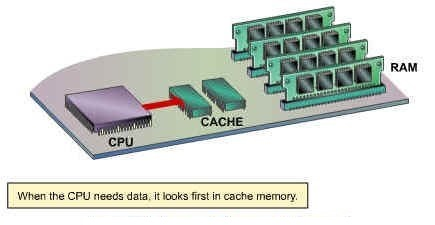
\includegraphics[scale = 0.72]{cacheonRAM.jpg} 
\end{frame}
 
% ========  1.1  =================
\begin{frame}
\frametitle{Coded Caching and Its Applications}
  \begin{itemize}
  \item A data management strategy to reduce delay during peak-traffic time,
  \item Single user setting, e.g. on-CPU caches, RAM in computers,
  \item Multiple user setting, e.g. networked system.
  \end{itemize}
  \vspace{0.5cm}
  \centering
  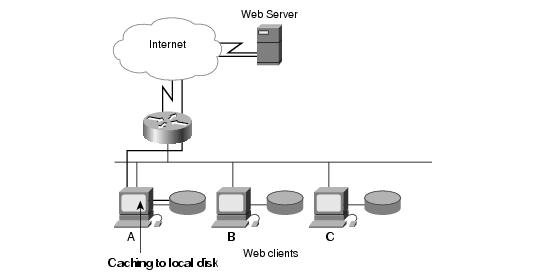
\includegraphics[scale = 0.6]{networkCaching.jpg} 
\end{frame}

% ========  2  =================
\begin{frame}
\frametitle{An Information-theoretic Formulation}
	\begin{itemize}
	\item $N$ files of same size, $K$ users, each with a local cache of size $M$,
	\item Prefetching phase: users fill their cache without knowing the requests,
	\item Delivery phase: each user requests a single file, server multicasts information to accommodate the requests.
	\end{itemize}
	\centering
	\includegraphics[scale = 0.3]{cacheNetwork.png}
\end{frame}

% ========  3  =================
\begin{frame}
\frametitle{Existing Schemes Using Uncoded Prefetching}
Maddah-Ali \& Niesen\footnotemark, improved by Yu et al\footnotemark, proved being optimal,
\begin{itemize}
\item Prefetching strategy:
	\begin{itemize}
	\setbeamertemplate{itemize items}[circle]
	\item Partition each file into $\binom{K}{t}$ segments, each associated with a cardinality-$t$ subset,
	\item Each user caches $\binom{K-1}{t-1}$ segments,
	\item E.g.: $(N,K) = (3,4), t = 2$,
	\end{itemize}
\vspace*{-15pt}
\begin{table}[]
\centering
\begin{tabular}{|l||l|l|l|l|l|l|l|l|l|}
\hline
User 1 & $A_{12}$ & $A_{13}$ & $A_{14}$ & $B_{12}$ & $B_{13}$ & $B_{14}$ & $C_{12}$ & $C_{13}$ & $C_{14}$ \\ \hline
User 2 & $A_{12}$ & $A_{23}$ & $A_{24}$ & $B_{12}$& $B_{23}$ & $B_{24}$ & $C_{12}$ & $C_{23}$ & $C_{24}$ \\ \hline
User 3 & $A_{13}$ & $A_{23}$ & $A_{34}$ & $B_{13}$ & $B_{23}$ & $B_{34}$ & $C_{13}$ & $C_{23}$ & $C_{34}$ \\ \hline
User 4 & $A_{14}$ & $A_{24}$ & $A_{34}$ & $B_{14}$ & $B_{24}$ & $B_{34}$ & $C_{14}$ & $C_{24}$ & $C_{34}$ \\ \hline
\end{tabular}
\end{table}
\item Delivery strategy
	\begin{itemize}
	\setbeamertemplate{itemize items}[circle]
	\item For any $(t+1)$ users subset $\mathcal{B}$, send the XOR of requested segments.
	\end{itemize}
\end{itemize}
\footnotetext[1]{\tiny Maddah-Ali M A, Niesen U. Fundamental limits of caching[J]. IEEE Transactions on Information Theory, 2014, 60(5): 2856-2867.}
\footnotetext[2]{\tiny Yu Q, Maddah-Ali M A, Avestimehr A S. The exact rate-memory tradeoff for caching with uncoded prefetching[J]. IEEE Transactions on Information Theory, 2017.}
\end{frame}


% ========  3.1  =================
\begin{frame}
\frametitle{Existing Schemes Using Uncoded Prefetching}
\begin{itemize}
\item Server transmits:
\begin{align*}
& \mathcal{B}=\{1,2,3\}:A_{23} +A_{13}+B_{12}, \;  \mathcal{B}=\{1,2,4\}:A_{24} +A_{14}+C_{12} \\
& \mathcal{B}=\{1,3,4\}:A_{34} +B_{14}+C_{13} ,\;  \mathcal{B}=\{2,3,4\}:A_{34} +B_{24}+C_{23}
\end{align*}
\end{itemize}
Using a brief moment, let's look at the decoding steps for the 1st user, when demand is (A,A,B,C):
\end{frame}

% ========  3.2  =================
\begin{frame}
\frametitle{Existing Schemes Using Uncoded Prefetching}
\begin{itemize}
\item Demand (A,A,B,C), server transmits:
\begin{align*}
& \textcolor{blue}{A_{23}} +\alert{A_{13}+B_{12}}, \quad  A_{24} +A_{14}+C_{12} \\
& A_{34} +B_{14}+C_{13} ,\quad  A_{34} +B_{24}+C_{23}
\end{align*}
\begin{table}[]
\centering
\begin{tabular}{|l||l|l|l|l|l|l|l|l|l|}
\hline
User 1 & $A_{12}$ & $\alert{A_{13}}$ & $A_{14}$ & $\alert{B_{12}}$ & $B_{13}$ & $B_{14}$ & $C_{12}$ & $C_{13}$ & $C_{14}$ \\ \hline
User 2 & $A_{12}$ & $A_{23}$ & $A_{24}$ & $B_{12}$ & $B_{23}$ & $B_{24}$ & $C_{12}$ & $C_{23}$ & $C_{24}$ \\ \hline
User 3 & $A_{13}$ & $A_{23}$ & $A_{34}$ & $B_{13}$ & $B_{23}$ & $B_{34}$ & $C_{13}$ & $C_{23}$ & $C_{34}$ \\ \hline
User 4 & $A_{14}$ & $A_{24}$ & $A_{34}$ & $B_{14}$ & $B_{24}$ & $B_{34}$ & $C_{14}$ & $C_{24}$ & $C_{34}$ \\ \hline
\end{tabular}
\end{table}
\end{itemize}
Step 1: using \alert{$A_{13}$} and \alert{$B_{12}$} to decode \textcolor{blue}{$A_{23}$};
\end{frame}

% ======== 3.3  =================
\begin{frame}
\frametitle{Existing Schemes Using Uncoded Prefetching}
\begin{itemize}
\item Demand (A,A,B,C), server transmits:
\begin{align*}
& \textcolor{blue}{A_{23}} +\alert{A_{13}+B_{12}}, \quad  \textcolor{blue}{A_{24}} +\alert{A_{14}}+\alert{C_{12}} \\
& A_{34} +B_{14}+C_{13} ,\quad  A_{34} +B_{24}+C_{23}
\end{align*}
\begin{table}[]
\centering
\begin{tabular}{|l||l|l|l|l|l|l|l|l|l|}
\hline
User 1 & $A_{12}$ & $\alert{A_{13}}$ & $\alert{A_{14}}$ & $\alert{B_{12}}$ & $B_{13}$ & $B_{14}$ & $\alert{C_{12}}$ & $C_{13}$ & $C_{14}$ \\ \hline
User 2 & $A_{12}$ & $A_{23}$ & $A_{24}$ & $B_{12}$ & $B_{23}$ & $B_{24}$ & $C_{12}$ & $C_{23}$ & $C_{24}$ \\ \hline
User 3 & $A_{13}$ & $A_{23}$ & $A_{34}$ & $B_{13}$ & $B_{23}$ & $B_{34}$ & $C_{13}$ & $C_{23}$ & $C_{34}$ \\ \hline
User 4 & $A_{14}$ & $A_{24}$ & $A_{34}$ & $B_{14}$ & $B_{24}$ & $B_{34}$ & $C_{14}$ & $C_{24}$ & $C_{34}$ \\ \hline
\end{tabular}
\end{table}
\end{itemize}
Step 2: using \alert{$A_{14}$} and \alert{$C_{12}$} to decode \textcolor{blue}{$A_{24}$};
\end{frame}


% ========  3.4  =================
\begin{frame}
\frametitle{Existing Schemes Using Uncoded Prefetching}
\begin{itemize}
\item Demand (A,A,B,C), server transmits
\begin{align*}
& \textcolor{blue}{A_{23}} +\alert{A_{13}+B_{12}}, \quad  \textcolor{blue}{A_{24}} +\alert{A_{14}}+\alert{C_{12}} \\
& \textcolor{blue}{A_{34}} +\alert{B_{14}}+\alert{C_{13}} ,\quad  A_{34} +B_{24}+C_{23}
\end{align*}
\begin{table}[]
\centering
\begin{tabular}{|l||l|l|l|l|l|l|l|l|l|}
\hline
User 1 & $A_{12}$ & $\alert{A_{13}}$ & $\alert{A_{14}}$ & $\alert{B_{12}}$ & $B_{13}$ & $\alert{B_{14}}$ & $\alert{C_{12}}$ & $\alert{C_{13}}$ & $C_{14}$ \\ \hline
User 2 & $A_{12}$ & $A_{23}$ & $A_{24}$ & $B_{12}$ & $B_{23}$ & $B_{24}$ & $C_{12}$ & $C_{23}$ & $C_{24}$ \\ \hline
User 3 & $A_{13}$ & $A_{23}$ & $A_{34}$ & $B_{13}$ & $B_{23}$ & $B_{34}$ & $C_{13}$ & $C_{23}$ & $C_{34}$ \\ \hline
User 4 & $A_{14}$ & $A_{24}$ & $A_{34}$ & $B_{14}$ & $B_{24}$ & $B_{34}$ & $C_{14}$ & $C_{24}$ & $C_{34}$ \\ \hline
\end{tabular}
\end{table}
\end{itemize}
Step 3: using \alert{$B_{14}$} and \alert{$C_{13}$} to decode \textcolor{blue}{$A_{34}$}; \\
User 1 now decodes the entire file A.
\end{frame}

% ========  4 =================
\begin{frame}
\frametitle{Existing Schemes Using Coded Prefetching}
Tian-Chen scheme\footnotemark[1],
\begin{itemize}
\item Prefetching strategy: 
	\begin{itemize}
	\setbeamertemplate{itemize items}[circle]
	\item A file is partitioned into $\binom{K}{t}$ segments, each user allocated $\binom{K-1}{t-1}$ segments,
	\item User encodes file segments using a rank metric code and stores the parities,
	\item E.g.: $(N,K) = (3,4), t = 2$, user 1 caches
	\end{itemize}
\begin{align*}
& \begin{pmatrix}
    \cdot   & \cdot  & \cdot  & \cdot &\cdot   & \cdot  & \cdot  & \cdot & \cdot \\
    \cdot   & \cdot  & \cdot  & \cdot &\cdot   & \cdot  & \cdot  & \cdot & \cdot \\
   \cdot   & \cdot  & \cdot  & \cdot &\cdot   & \cdot  & \cdot  & \cdot & \cdot \\
    \cdot   & \cdot  & \cdot  & \cdot &\cdot   & \cdot  & \cdot  & \cdot & \cdot \\
    \cdot   & \cdot  & \cdot  & \cdot &\cdot   & \cdot  & \cdot  & \cdot & \cdot 
\end{pmatrix}_{(5 \times 9)}
\cdot \\
& (A_{12},A_{13},A_{14},B_{12},B_{13},B_{14},C_{12},C_{13},C_{14})^T
\end{align*}
In the example, a (14,9) systematic rank metric code is used, user 1 stores the 5 parities.
\end{itemize}
\footnotetext[1]{\tiny Tian C, Chen J. Caching and delivery via interference elimination[C]. Information Theory (ISIT), 2016 IEEE International Symposium on. IEEE, 2016: 830-834.}
\end{frame}


% ========  4.1 =================
\begin{frame}
\frametitle{Existing Schemes Using Coded Prefetching}
\begin{itemize}
\item Delivery strategy: Linear combination of segments from one file.
\begin{itemize}
	\setbeamertemplate{itemize items}[circle]
	\item E.g.: demand (A,A,B,C), transmits 9 (coded) symbols:
	\begin{align*}
	A_{34}, B_{12}, B_{14}, B_{24}, C_{12},C_{13},C_{23},A_{13}+A_{23},A_{14}+A_{24}
	\end{align*}
	\item Each symbol serves two roles: \\
	1) content delivery for some users; \\
	2) help resolve coded symbols for some other users. 
	\end{itemize}
\end{itemize}
To be clear, let's check user 1,
\end{frame}

% ========  4.2 =================
\begin{frame}
\frametitle{Existing Schemes Using Coded Prefetching}
\begin{itemize}
\item Demand (A,A,B,C), server transmits:
\begin{align*}
A_{34}, \textcolor{blue}{B_{12}, B_{14}}, B_{24}, \textcolor{blue}{C_{12},C_{13}}, C_{23},A_{13}+A_{23},A_{14}+A_{24}
\end{align*}
\end{itemize}
\vspace{-10pt}
\begin{align*}
& \begin{pmatrix}
    \cdot   & \cdot  & \cdot  & \cdot &\cdot   & \cdot  & \cdot  & \cdot & \cdot \\
    \cdot   & \cdot  & \cdot  & \cdot &\cdot   & \cdot  & \cdot  & \cdot & \cdot \\
   \cdot   & \cdot  & \cdot  & \cdot &\cdot   & \cdot  & \cdot  & \cdot & \cdot \\
    \cdot   & \cdot  & \cdot  & \cdot &\cdot   & \cdot  & \cdot  & \cdot & \cdot \\
    \cdot   & \cdot  & \cdot  & \cdot &\cdot   & \cdot  & \cdot  & \cdot & \cdot \\
               &           &          &  \textcolor{blue}{\cdot} &         &         &         &           &       \\
                   &            &            &           &            & \textcolor{blue}{\cdot}  &            &   &   \\
                    &            &            &           &            &            & \textcolor{blue}{\cdot}  &   &   \\
                         &            &            &           &            &            &            & \textcolor{blue}{\cdot} &          
\end{pmatrix}_{(5 \times 9)}
\cdot \\
& (A_{12},A_{13},A_{14},B_{12},B_{13},B_{14},C_{12},C_{13},C_{14})^T
\end{align*}
Step 1: user 1 collects 4 symbols \textcolor{blue}{$B_{12}, B_{14},C_{12},C_{13}$};\\
Together with 5 (coded) symbols in his cache, he can decode all 9 symbols.
\end{frame}

% ========  4.3 =================
\begin{frame}
\frametitle{Existing Schemes Using Coded Prefetching}
\begin{itemize}
\item Demand (A,A,B,C), server transmits:
\begin{align*}
\textcolor{blue}{A_{34}}, B_{12}, B_{14}, B_{24}, C_{12},C_{13}, C_{23}, \textcolor{red}{A_{13}}+\textcolor{blue}{A_{23}},\textcolor{red}{A_{14}}+\textcolor{blue}{A_{24}}
\end{align*}
\end{itemize}
Step 2: user 1 already resolved all symbols in the cache, as following:
\begin{table}[]
\centering
\begin{tabular}{|l||l|l|l|l|l|l|l|l|l|}
\hline
User 1 & $A_{12}$ & $\textcolor{red}{A_{13}}$ & $\textcolor{red}{A_{14}}$ & $B_{12}$ & $B_{13}$ & $B_{14}$ & $C_{12}$ & $C_{13}$ & $C_{14}$ \\ \hline
\end{tabular}
\end{table}
He then collects $\textcolor{red}{A_{13}}+\textcolor{blue}{A_{23}},\textcolor{red}{A_{14}}+\textcolor{blue}{A_{24}}$, he can decode \textcolor{blue}{$A_{23}, A_{24}$};
\end{frame}

% ========  4.4 =================
\begin{frame}
\frametitle{Existing Schemes Using Coded Prefetching}
\begin{itemize}
\item Demand (A,A,B,C), server transmits:
\begin{align*}
\textcolor{blue}{A_{34}}, B_{12}, B_{14}, B_{24}, C_{12},C_{13}, C_{23}, A_{13}+A_{23},A_{14}+A_{24}
\end{align*}
\end{itemize}
Step 3: user 1 collects $\textcolor{blue}{A_{34}}$, now he decodes the entire file A;
\end{frame}


% ========  5  =================
\begin{frame}
\frametitle{Two Quite Different Schemes}
\begin{itemize}
\item Uncoded prefetching \textit{vs.} coded prefetching,
\item Binary code \textit{vs.} non-binary code,
\item Encoding/decoding using simple combinatorics \textit{vs.} sophisticated coding techniques (rank metric codes),
\item Uncoded prefetching performs better at high cache memory regime \textit{vs.} coded prefetching performs better at low cache memory regime.
\end{itemize}
\centering
\textit{Largely unrelated... }\\
\textit{Are there any connections?}
\end{frame}

% ========  5  =================
\begin{frame}
\frametitle{Some Backgrounds}
\begin{itemize}
\item Linearized Polynomial:
A degree-$q^{P-1}$ linearized polynomial in the finite field $\mathbb{F}_{q^m}$
\begin{equation}
f(x) = \sum_{i = 1,2,\ldots, P} v_i x^{q^{i-1}}, v_i \in \mathbb{F}_{q^m}
\end{equation}
can be uniquely identified from evaluations at any $P$ points $x = \theta_{i} \in \mathbb{F}_{q^m}, i = 1,2,\ldots, P$, that are linearly independent over $\mathbb{F}_q$.
\end{itemize}
\end{frame}

%========  5.1 =================
\begin{frame}
\frametitle{Some Backgrounds}
\begin{block}{Lemma}
Let $f(x)$ be a degree-$q^{P-1}$ linearized polynomial in $\mathbb{F}_{q^m}$, and $\theta_i \in \mathbb{F}_{q^m}, i = 1,2,\ldots,P_o$, be linearly independent over $\mathbb{F}_q$. Let $G$ be a $P_o \times P$ full rank (rank $P$) matrix with entries in $\mathbb{F}_q$, then $f(x)$ can be  uniquely identified from 
\begin{equation}
[f(\theta_1), f(\theta_2), \ldots, f(\theta_{P_o})] \cdot G.
\end{equation}
\end{block}

\setbeamertemplate{itemize items}[circle]
\begin{itemize}
\item $(v_1,\ldots, v_P)$ are information symbols to be encoded; $[f(\theta_1),\ldots,f(\theta_{P_o})]$ are coded symbols;
\item A $(P_o,P)$ MDS code in terms of rank metric.
\end{itemize}
\end{frame}

% ========  6 =================
\begin{frame}
\frametitle{A Hidden Connection}
Continuing example $(N,K)=(3,4), t=2$, demand = (A,A,B,C):

\begin{itemize}
\item Yu et al scheme transmits (4 symbols):
\begin{align*}
& A_{23} +A_{13}+B_{12}, \quad  A_{24} +A_{14}+C_{12} \\
& A_{34} +B_{14}+C_{13} ,\quad  A_{34} +B_{24}+C_{23}
\end{align*}
\end{itemize}
\centering
Separate different files \& remove repeated transmissions, \\
$\Downarrow$
\begin{itemize}
\item Tian-Chen scheme (9 symbols):
\begin{align*}
& A_{23} +A_{13}, \quad B_{12}, \qquad  A_{24} +A_{14}, \quad C_{12} \\
& A_{34}, \quad B_{14}, \quad C_{13}, \qquad  \qquad \quad B_{24}, \quad C_{23}
\end{align*}
\end{itemize}
Instead of fully decomposing a transmission, what if we partially decompose them?
\end{frame}


% ========  6.1 =================
\begin{frame}
\frametitle{An Alternative Scheme}
\begin{itemize}
\item A partial decomposition: deliver 5 coded symbols:
	\begin{itemize}
	\setbeamertemplate{itemize items}[circle]
	\item Demand (A,A,B,C), transmits
	\begin{align*}
	& A_{23} +A_{13}+B_{12}, \quad  A_{24} +A_{14}+C_{12} \\
	& A_{34}, \quad B_{14}+C_{13} ,\qquad \qquad B_{24}+C_{23}
	\end{align*}
	\item Demand (A,A,B,B), transmits
	\begin{align*}
	& A_{23} +A_{13}+B_{12}, \quad  A_{24} +A_{14}+B_{12} \\
	& A_{34}, \quad B_{14}+B_{13} ,\qquad \qquad B_{24}+B_{23}
	\end{align*}
	\end{itemize}
\end{itemize}
\end{frame}

% ========  6.2 =================
\begin{frame}
\frametitle{An Alternative Scheme}

\begin{itemize}
\item A partial decomposition: deliver 5 coded symbols:
	\begin{itemize}
	\setbeamertemplate{itemize items}[circle]
	\item Demand (A,A,A,C), transmits
	\begin{align*}
	& A_{23} +A_{13}+A_{12}, \quad  A_{24} +A_{14}+C_{12} \\
	& A_{34}, \quad A_{14}+C_{13} ,\qquad \qquad A_{24}+C_{23}
	\end{align*}
	\item Demand (A,A,A,A), transmits
	\begin{align*}
	& A_{23} +A_{13}+A_{12}, \quad  A_{24} +A_{14}+A_{12} \\
	& A_{34}, \quad A_{14}+A_{13} ,\qquad \qquad A_{24}+A_{23}
	\end{align*}
	\end{itemize}
\end{itemize}
\end{frame}


% ========  6.3 =================
\begin{frame}
\frametitle{An Alternative Scheme}
\begin{itemize}
\item Each user only needs to cache 8 linear combinations,
\item Every transmission could have different ways to be partially decomposed, i.e. \textit{decomposition pattern}s,
\item Above is a good choice of decomposing, in fact produces a new corner point at $(M,R)=(4/3,5/6)$.
\end{itemize}
We will give a generalized scheme and code examples.
\end{frame}

% ========  7  =================
\begin{frame}
\frametitle{Partial Decomposition and A New Code Example}
To facilitate understanding, we introduce some notions:
\begin{itemize}
\item \textcolor{blue}{Demand vector} $\boldsymbol{d}=\{d_1,\ldots,d_K\}$ denotes the demands by $K$ users, $d_k \in [1:N]$,
\item Each transmission in Yu scheme can be represented as 
\begin{equation*}
\oplus_{k \in \mathcal{B}}W_{d_k,\mathcal{B} \backslash k},  \quad |\mathcal{B}|=t+1,
\end{equation*}
a \textcolor{blue}{transmission type} $\boldsymbol{t}=(t_1,\ldots,t_N)$ is associated with a transmission where $t_n$ denotes the number of users in subset $|\mathcal{B}|$ requesting file $W_n$. Set $\mathcal{T}_{\boldsymbol{d}}^{(t)}$ denotes all valid transmission types for a demand $\boldsymbol{d}$.
\end{itemize}
\end{frame}

% ========  7.1  =================
\begin{frame}
\frametitle{Partial Decomposition and A New Code Example}
\begin{itemize}
	\item A \textcolor{blue}{partial decomposition} $\mathcal{P}_{\boldsymbol{t},\boldsymbol{d}}$ of transmission type $\boldsymbol{t}$ is a partition of $\mathbb{supp}(\boldsymbol{t})$. The full set of decomposition patterns is $\boldsymbol{\mathcal{P}}_{\boldsymbol{d}}^{(t)}= \{\mathcal{P}_{\boldsymbol{t},\boldsymbol{d}} | \boldsymbol{t} \in \mathcal{T}_{\boldsymbol{d}}^{(t)}\}$.
	\item The collection of all possible $\mathcal{P}_{\boldsymbol{t},\boldsymbol{d}}$ is $\mathfrak{P}_{\boldsymbol{t},\boldsymbol{d}}$.
	\item E.g.: $(N,K)=(3,4), t=2,\boldsymbol{d}=(1,1,2,3)$,
	$\mathcal{T}_{\boldsymbol{d}}^{(t)}= \{(2,1,0), (2,0,1),(1,1,1)\}$, for $\boldsymbol{t}=(1,1,1)$:
\vspace{-10pt}
\begin{align*}
& \mathcal{B}=\{1,3,4\}: A_{34}+B_{14}+C_{13}  \;  \xrightarrow[]{\text{decompose}} \; \{A_{34}, B_{14}+C_{13} \}\\
&  \mathcal{B}=\{2,3,4\}: A_{34}+B_{24}+C_{23}  \; \quad \qquad  \qquad \{A_{34}, B_{24}+C_{23}\}
\end{align*}
Decomposition pattern $\mathcal{P}_{\boldsymbol{t},\boldsymbol{d}}=\mathcal{P}_{(1,1,1)(1,1,2,3)}=\{\{1\}, \{2,3\}\}$.
\end{itemize}
\end{frame}

% ========  8  =================
\begin{frame}
\frametitle{Partial Decomposition and A New Code Example}
Partial decomposition could produce new memory-rate points:
\begin{itemize}
\item For each demand $\boldsymbol{d}$, using multiple coding instances,
\item Fix a decomposition pattern $\mathcal{P}_{\boldsymbol{t},\boldsymbol{d}}$ for each $\boldsymbol{t}$, 
\item Set an auxiliary variable $\alpha_{\boldsymbol{d},\boldsymbol{\mathcal{P}}_{\boldsymbol{d}}^{(t)}}$ for each decomposition pattern, s.t.
\begin{align*}
& \sum_{\boldsymbol{\mathcal{P}}_{\boldsymbol{d}}^{(t)} \in \mathfrak{P}_{\boldsymbol{t},\boldsymbol{d}}}\alpha_{\boldsymbol{d},\boldsymbol{\mathcal{P}}_{\boldsymbol{d}}^{(t)}}=1, \quad \boldsymbol{d} \in \mathcal{D}, \\
& 1 \geq \alpha_{\boldsymbol{d},\boldsymbol{\mathcal{P}}_{\boldsymbol{d}}^{(t)}} \geq 0, \quad \boldsymbol{d} \in \mathcal{D}, \quad \boldsymbol{\mathcal{P}}_{\boldsymbol{d}}^{(t)} \in \mathfrak{P}_{\boldsymbol{t},\boldsymbol{d}}.
\end{align*}
	\begin{itemize}
	\setbeamertemplate{itemize items}[circle]
	\item $\alpha_{\boldsymbol{d},\boldsymbol{\mathcal{P}}_{\boldsymbol{d}}^{(t)}}$: how much fraction of instances using a decomposition pattern;
	\item Intuitively same as ``time sharing", but not equivalent.
	\end{itemize}
\end{itemize}
\end{frame}


% ========  8.1  =================
\begin{frame}
\frametitle{Partial Decomposition and A New Code Example}
\begin{itemize}
\item Prefetching:
	\begin{itemize}
	\setbeamertemplate{itemize items}[circle]
	\item Partition each file into $r\binom{K}{t}$ segments ($r$ instances each of $\binom{K}{t}$ segments), each to be in $\mathbb{F}_{2^m}$ for sufficiently large $m$,
	\item Each user is allocated $P=rN\binom{K-1}{t-1}$ symbols; caches $P_o-P$ linear combinations:
	\begin{equation*}
	P_o-P=rM_r' \binom{K}{t}
	\end{equation*}
	($M_r'$ to be defined later)
	\item Using $(P_o,P)$ systematic rank metric code to encode $P$ symbols, caches the parities;
	\item $m \geq P_o$ suffices for existence of rank metric code.
	\end{itemize}
\end{itemize}
\end{frame}

% ========  8.2  =================
\begin{frame}
\frametitle{Partial Decomposition and A New Code Example}
\begin{itemize}
\item Delivery:
	\begin{itemize}
	\setbeamertemplate{itemize items}[circle]
	\item For demand $\boldsymbol{d}$ = (A,A,B,C)=(1,1,2,3), let $\alpha_{\boldsymbol{d},\boldsymbol{\mathcal{P}}_{\boldsymbol{d}}^{(t)}}=1$, $\boldsymbol{\mathcal{P}}_{\boldsymbol{d}}^{(t)}=\boldsymbol{\mathcal{P}}_{(1,1,2,3)}^{(2)}$ are: 
	\begin{align*}
	& \mathcal{P}_{(2,1,0),(1,1,2,3)} = \{\{1,2\}\} = \{\{A,B\}\}: A_{23} +A_{13} + B_{12},\\
	& \mathcal{P}_{(2,0,1),(1,1,2,3)} =  \{\{1,3\}\} = \{\{A,C\}\}: A_{24} +A_{14} + C_{12},\\
	& \mathcal{P}_{(1,1,1),(1,1,2,3)} = \{\{1\},\{2,3\}\} = \{\{A\},\{B,C\}\}: \\
	& \qquad \qquad  \qquad   A_{34}, \quad B_{14} + C_{13}, \ B_{24} + C_{23}
	\end{align*}
	Thus $R_{\boldsymbol{d},\boldsymbol{\mathcal{P}}_{\boldsymbol{d}}^{(t)}} = 5, M_{\boldsymbol{d},\boldsymbol{\mathcal{P}}_{\boldsymbol{d}}^{(t)},k} = 8$, for $k \in [1:4]$.
	\end{itemize}
\end{itemize}
\end{frame}

% ========  8.3  =================
\begin{frame}
\frametitle{Partial Decomposition and A New Code Example}
\begin{itemize}
\item Delivery:
	\begin{itemize}
	\setbeamertemplate{itemize items}[circle]
	\item For demand $\boldsymbol{d}$ = (A,A,B,B)=(1,1,2,2), two decomposition patterns: \\
	1st pattern: $\boldsymbol{\mathcal{P}}_{\boldsymbol{d}}^{(t)}$ without any decomposition, let $\alpha_{\boldsymbol{d},\boldsymbol{\mathcal{P}}_{\boldsymbol{d}}^{(t)}}=1/2$,
	\begin{align*}
	& A_{23}^{(1)} +A_{13}^{(1)}+B_{12}^{(1)}, \quad  A_{24}^{(1)} +A_{14}^{(1)}+B_{12}^{(1)} \\
	& A_{34}^{(1)} +B_{14}^{(1)}+B_{13}^{(1)} ,\quad  A_{34}^{(1)} +B_{24}^{(1)}+B_{23}^{(1)} 
	\end{align*}
	For this pattern, $R_{\boldsymbol{d},\boldsymbol{\mathcal{P}}_{\boldsymbol{d}}^{(t)}} = 4, M_{\boldsymbol{d},\boldsymbol{\mathcal{P}}_{\boldsymbol{d}}^{(t)},k} = 9, k \in [1:4]$.
	\end{itemize}
\end{itemize}
\end{frame}

% ========  8.4  =================
\begin{frame}
\frametitle{Partial Decomposition and A New Code Example}
\begin{itemize}
\item Delivery:
	\begin{itemize}
	\setbeamertemplate{itemize items}[circle]
	\item For demand $\boldsymbol{d}$ = (A,A,B,B)=(1,1,2,2), two decomposition patterns: \\
	2nd pattern: the following decompositions $\boldsymbol{\mathcal{P}}_{\boldsymbol{d}}^{(t)}$:
	\begin{align*}
	& \mathcal{P}_{(2,1,0),(1,1,2,2)} = \{\{1\},\{2\}\} = \{\{A\},\{B\}\}: A_{23}^{(2)}+A_{13}^{(2)}, B_{12}^{(2)}, \\
	& \qquad \qquad \qquad  \qquad \qquad \qquad \qquad \qquad \qquad \quad A_{24}^{(2)}+A_{14}^{(2)},B_{12}^{(2)}; \\
	& \mathcal{P}_{(1,2,0),(1,1,2,2)} =  \{\{1\},\{2\}\} = \{\{A\},\{B\}\}: A_{34}^{(2)}, B_{14}^{(2)} + B_{13}^{(2)},\\
	& \qquad \qquad \qquad  \qquad \qquad \qquad \qquad \qquad \qquad \quad  A_{34}^{(2)}, B_{24}^{(2)}+B_{23}^{(2)};
	\end{align*}
	For this pattern, $R_{\boldsymbol{d},\boldsymbol{\mathcal{P}}_{\boldsymbol{d}}^{(t)}} = 6, M_{\boldsymbol{d},\boldsymbol{\mathcal{P}}_{\boldsymbol{d}}^{(t)},k} = 7$, for $k \in [1:4]$.
	\end{itemize}
\end{itemize}
\end{frame}

% ========  8.5  =================
\begin{frame}
\frametitle{Partial Decomposition and A New Code Example}
\begin{itemize}
\item Delivery:
	\begin{itemize}
	\setbeamertemplate{itemize items}[circle]
	\item For demand $\boldsymbol{d}$ = (A,A,A,A)=(1,1,1,1), two decomposition patterns: \\
	1st pattern: $\boldsymbol{\mathcal{P}}_{\boldsymbol{d}}^{(t)}$ without any decomposition, let $\alpha_{\boldsymbol{d},\boldsymbol{\mathcal{P}}_{\boldsymbol{d}}^{(t)}}=5/6$,
	\begin{align*}
	& A_{23}^{(i)} +A_{13}^{(i)}+A_{12}^{(i)}, \quad  A_{24}^{(i)} +A_{14}^{(i)}+A_{12}^{(i)} \\
	& A_{34}^{(i)} +A_{14}^{(i)}+A_{13}^{(i)}, \quad \text{for} \; i = 1,2,3,4,5.
	\end{align*}
	For this pattern, $R_{\boldsymbol{d},\boldsymbol{\mathcal{P}}_{\boldsymbol{d}}^{(t)}} = 3, M_{\boldsymbol{d},\boldsymbol{\mathcal{P}}_{\boldsymbol{d}}^{(t)},k} = 9, k \in [1:4].$
	\end{itemize}
\end{itemize}
\end{frame}

% ========  8.6  =================
\begin{frame}
\frametitle{Partial Decomposition and A New Code Example}
\begin{itemize}
\item Delivery:
	\begin{itemize}
	\setbeamertemplate{itemize items}[circle]
	\item For demand $\boldsymbol{d}$ = (A,A,A,A)=(1,1,1,1), two decomposition patterns: \\
	2nd pattern: special uncoded decomposition pattern $\breve{\boldsymbol{\mathcal{P}}}_{\boldsymbol{d}}^{(t)}$, let $\alpha_{\boldsymbol{d},\boldsymbol{\mathcal{P}}_{\boldsymbol{d}}^{(t)}}=1/6$,
	\begin{align*}
	& A_{23}^{(6)}, A_{13}^{(6)}, A_{24}^{(6)}, A_{14}^{(6)}, A_{12}^{(6)}, A_{34}^{(6)} \\
	& B_{23}^{(6)}, B_{13}^{(6)}, B_{24}^{(6)}, B_{14}^{(6)}, B_{12}^{(6)}, B_{34}^{(6)} 
	\end{align*}
	For this pattern, $R_{\boldsymbol{d},\boldsymbol{\mathcal{P}}_{\boldsymbol{d}}^{(t)}} = 12, M_{\boldsymbol{d},\boldsymbol{\mathcal{P}}_{\boldsymbol{d}}^{(t)},k} = 3, k \in [1:4].$
	\end{itemize}
\end{itemize}
\end{frame}

% ========  8.7 =================
\begin{frame}
\frametitle{Partial Decomposition and A New Code Example}
\begin{itemize}
\item The above example uses $r=6$ instances of code,
\item Of all 6 instances, $r_{\boldsymbol{d},\boldsymbol{\mathcal{P}}_{\boldsymbol{d}}^{(t)}}$ of them adopt decomposition $\boldsymbol{\mathcal{P}}_{\boldsymbol{d}}^{(t)}$, 
\item Memory-rate pair 
\begin{equation*}
(M,R)=\frac{1}{r\binom{K}{t}} \Bigg( \sum_{\boldsymbol{\mathcal{P}}_{\boldsymbol{d}}^{(t)}} r_{\boldsymbol{d},\boldsymbol{\mathcal{P}}_{\boldsymbol{d}}^{(t)}} M_{\boldsymbol{d},\boldsymbol{\mathcal{P}}_{\boldsymbol{d}}^{(t)},k}, \sum_{\boldsymbol{\mathcal{P}}_{\boldsymbol{d}}^{(t)}} r_{\boldsymbol{d},\boldsymbol{\mathcal{P}}_{\boldsymbol{d}}^{(t)}} R_{\boldsymbol{d},\boldsymbol{\mathcal{P}}_{\boldsymbol{d}}^{(t)}} \Bigg)
\end{equation*}
would be \\
\centering 
$(M,R)=(4/3, 5/6)$.
\end{itemize}
\end{frame}

% ========  9 =================
\begin{frame}
\frametitle{A New Information-Theoretic Inner Bound}
\begin{figure}[]
\centering
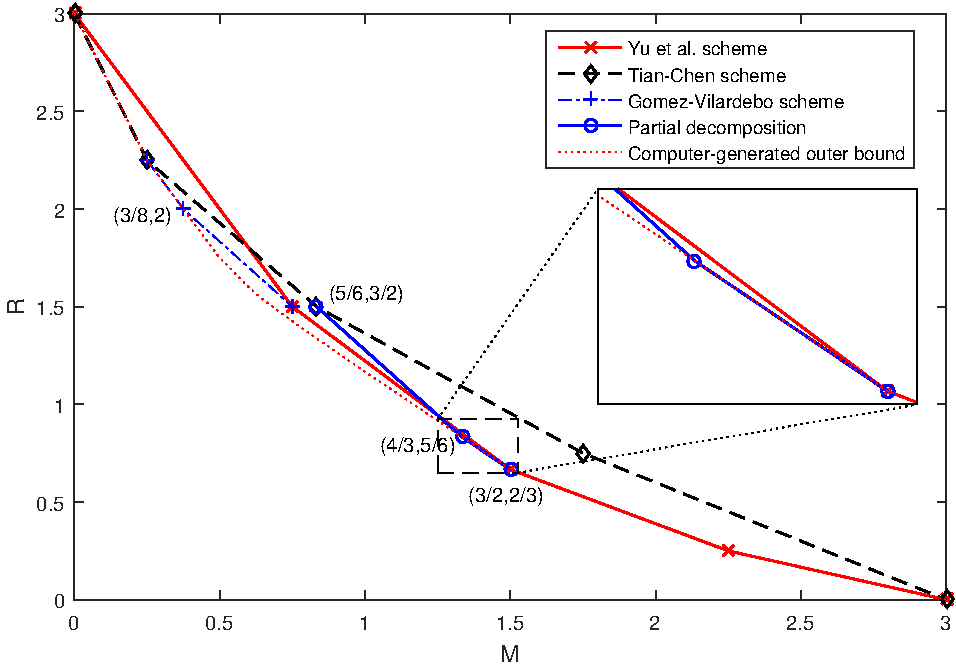
\includegraphics[width=8.5cm]{plot34.pdf}
\caption{\label{fig:system}A new information-theoretic inner-bound for the example caching system $(N,K)=(3,4), t=2$.}
\end{figure}
\end{frame}

% ========  10  =================
\begin{frame}
\frametitle{A New Information-Theoretic Inner Bound}
\begin{itemize}
\item For some demands, special uncoded transmission needed to keep the decomposition rule;
\item As the parameters increase, number of decomposition patterns for each $\boldsymbol{t}$ grows; 
\item The best decompositions for all $\boldsymbol{t}$? Exhaustive search, practically impossible to calculate by hand;
\item We can use a computer-aided approach.
\end{itemize}
Before the details, we show a new corner point for caching system $(N,K)=(4,8), t=2$.
\vspace{20pt}

\centering
This time it is calculated using a computer program.
\end{frame}

% ========  11  =================
\begin{frame}
\frametitle{A New Information-Theoretic Inner Bound}
\begin{figure}[]
\centering
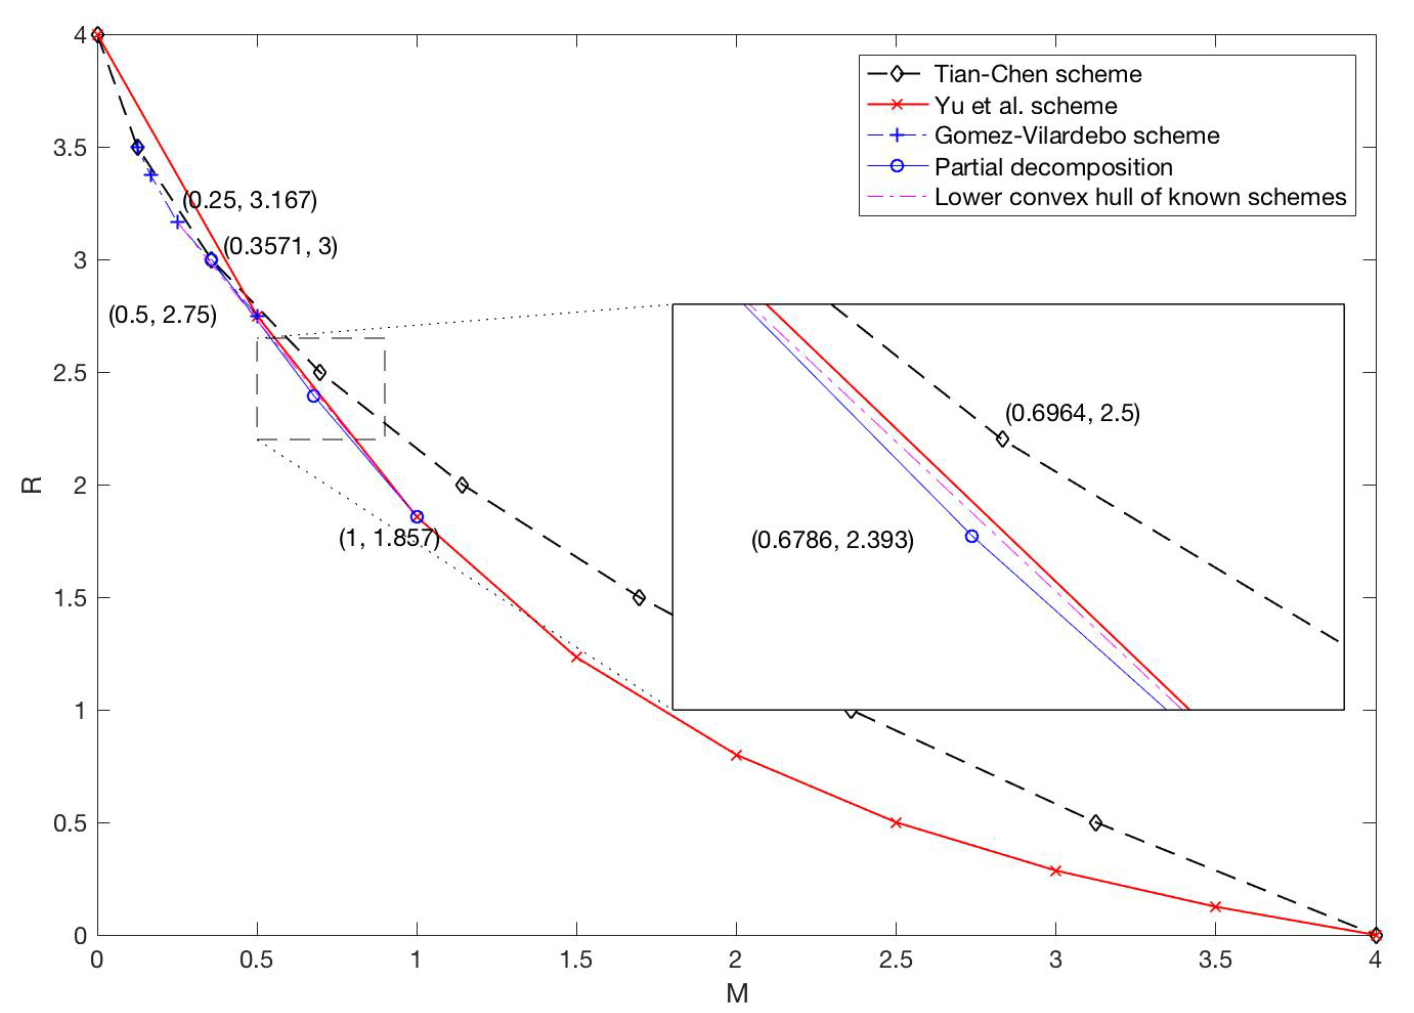
\includegraphics[width=8.5cm]{plot48.pdf}
\caption{\label{fig:system}A new information-theoretic inner-bound for the example caching system $(N,K)=(4,8), t=2$.}
\end{figure}
\end{frame}
% ========  12  =================
\begin{frame}
\frametitle{A Linear Programming Framework}
The inner-bound of the new coding scheme can be calculated using linear programming:
\begin{itemize}
\item Define rate region $\mathcal{R}^{(t)}$: collection of memory-rate pairs $(M,R)$ such that exists set of $\{\alpha_{\boldsymbol{d},\boldsymbol{\mathcal{P}}_{\boldsymbol{d}}^{(t)}}\}$ satisfying
\begin{align*}
& \scalemath{0.8}{\sum_{\boldsymbol{\mathcal{P}}_{\boldsymbol{d}}^{(t)} \in \mathfrak{P}_{\boldsymbol{t},\boldsymbol{d}}}\alpha_{\boldsymbol{d},\boldsymbol{\mathcal{P}}_{\boldsymbol{d}}^{(t)}}=1, \quad \boldsymbol{d} \in \mathcal{D}}, \\
& \scalemath{0.8}{1 \geq \alpha_{\boldsymbol{d},\boldsymbol{\mathcal{P}}_{\boldsymbol{d}}^{(t)}} \geq 0, \quad \boldsymbol{d} \in \mathcal{D}, \quad \boldsymbol{\mathcal{P}}_{\boldsymbol{d}}^{(t)} \in \mathfrak{P}_{\boldsymbol{t},\boldsymbol{d}}}, \\
& \scalemath{0.8}{\sum_{\boldsymbol{\mathcal{P}}_{\boldsymbol{d}}^{(t)} \in \mathfrak{P}_{\boldsymbol{t},\boldsymbol{d}}} \alpha_{\boldsymbol{d},\boldsymbol{\mathcal{P}}_{\boldsymbol{d}}^{(t)}} R_{\boldsymbol{d},\boldsymbol{\mathcal{P}}_{\boldsymbol{d}}^{(t)}} \leq R\binom{K}{t}, \quad \boldsymbol{d} \in \mathcal{D}}, \\
& \scalemath{0.8}{\sum_{\boldsymbol{\mathcal{P}}_{\boldsymbol{d}}^{(t)} \in \mathfrak{P}_{\boldsymbol{t},\boldsymbol{d}}} \alpha_{\boldsymbol{d},\boldsymbol{\mathcal{P}}_{\boldsymbol{d}}^{(t)}} M_{\boldsymbol{d},\boldsymbol{\mathcal{P}}_{\boldsymbol{d}}^{(t)}} \leq M\binom{K}{t}, \quad \boldsymbol{d} \in \mathcal{D}, k \in [1:K]}.
\end{align*}
\end{itemize}
\end{frame}
%
% ========  13  =================
\begin{frame}
\frametitle{A Linear Programming Framework}
The inner-bound of the new coding scheme can be calculated using linear programming:
\begin{itemize}
\item Further define 
\begin{equation*}
(M_{\boldsymbol{d}}', R_{\boldsymbol{d}}') =\frac{1}{r\binom{K}{t}} \Bigg( \max_{k \in [1:K]}\sum_{\boldsymbol{\mathcal{P}}_{\boldsymbol{d}}^{(t)}} r_{\boldsymbol{d},\boldsymbol{\mathcal{P}}_{\boldsymbol{d}}^{(t)}} M_{\boldsymbol{d},\boldsymbol{\mathcal{P}}_{\boldsymbol{d}}^{(t)},k}, \sum_{\boldsymbol{\mathcal{P}}_{\boldsymbol{d}}^{(t)}} r_{\boldsymbol{d},\boldsymbol{\mathcal{P}}_{\boldsymbol{d}}^{(t)}} R_{\boldsymbol{d},\boldsymbol{\mathcal{P}}_{\boldsymbol{d}}^{(t)}} \Bigg)
\end{equation*}
and 
\begin{equation*}
M_r' \triangleq \max_{\boldsymbol{d} \in \mathcal{D}} M_{\boldsymbol{d}}', \qquad R_r' \triangleq \max_{\boldsymbol{d} \in \mathcal{D}} R_{\boldsymbol{d}}' .
\end{equation*}
\end{itemize}
\end{frame}

% ========  14  =================
\begin{frame}
\frametitle{A Linear Programming Approach}
The inner-bound of the new coding scheme can be calculated using linear programming:
\begin{itemize}
\item The number of instances $r$ can be chosen s.t. exists $\{r_{\boldsymbol{d},\boldsymbol{\mathcal{P}}_{\boldsymbol{d}}^{(t)}}\}$ 
\begin{equation*}
\left|\frac{r_{\boldsymbol{d},\boldsymbol{\mathcal{P}}_{\boldsymbol{d}}^{(t)}}}{r}-\alpha_{\boldsymbol{d},\boldsymbol{\mathcal{P}}_{\boldsymbol{d}}^{(t)}}\right| \leq \epsilon.
\end{equation*}
By making $r$ large and choosing appropriate $\{r_{\boldsymbol{d},\boldsymbol{\mathcal{P}}_{\boldsymbol{d}}^{(t)}}\}$ s.t. $\epsilon \geq 0$ being arbitrarily small. We have 
\begin{equation*}
\lim_{r \rightarrow \infty}(M_r', R_r')=(M,R),
\end{equation*}
it will be the effective memory-rate pair of the new code.
\end{itemize}
\end{frame}

% ========  15  =================
\begin{frame}
\frametitle{Conclusion}
\begin{itemize}
\item A single scheme unifying two general classes of schemes (uncoded and coded),
\item The Yu et al scheme and Tian-Chen scheme are two extreme points of the new scheme,
\item The notion of Transmission type plays an important role and is overlooked before this work, 
\item The performance improvement is not quite large, and mostly reside in the middle $M$ regime, which are not surprise.
\end{itemize}
\end{frame}

% ========  16  =================
\begin{frame}
\frametitle{Conclusion}
\begin{itemize}
\item The new coding scheme can not incorporate the coding scheme of G{\'o}mez-Vilardeb{\'o}\footnotemark[1], a more generalized code may exist?
\item The complexity: certain decomposing patterns are obviously bad choice; Simplifying the proposed scheme appears worthwhile.
\end{itemize}
\footnotetext[1]{\tiny  J.~G{\'o}mez-Vilardeb{\'o}, ``Fundamental limits of caching: Improved bounds with coded prefetching,'' \emph{arXiv:1612.09071}, Dec. 2016.}
\end{frame}

\end{document}